%%%%%%%%%%%%%%%%%%%%%%%%%%%%%%%%%%%%%%%%%%%%%%%%%%%%%%%%%%%%%%%%%%%
%  File name: ch5-Stats.tex
%  Title:
%  Version: 20.06.2019 (hve)
%%%%%%%%%%%%%%%%%%%%%%%%%%%%%%%%%%%%%%%%%%%%%%%%%%%%%%%%%%%%%%%%%%%
%%%%%%%%%%%%%%%%%%%%%%%%%%%%%%%%%%%%%%%%%%%%%%%%%%%%%%%%%%%%%%%%%%%
\chapter[Descriptive linear regression analysis]{\href{https://www.youtube.com/watch?v=uMpJZ2g0e3E}{Descriptive linear regression analysis}}
\lb{ch5}
%%%%%%%%%%%%%%%%%%%%%%%%%%%%%%%%%%%%%%%%%%%%%%%%%%%%%%%%%%%%%%%%%%%
For strongly correlating bivariate sample data 
$\{(x_{i},y_{i})\}_{i=1,\ldots,n}$ for a metrically scaled 
two-dimensional statistical variable~$(X,Y)$, i.e., when $0.71 
\leq |r| \leq 1.0$, it is meaningful to construct a mathematical 
model of the linear quantitative statistical association so 
diagnosed. The standard method to realise this by systematic means 
is due to the German mathematician and astronomer 
\href{http://www-groups.dcs.st-and.ac.uk/~history/Biographies/Gauss.html}{Carl Friedrich Gau\ss\ (1777--1855)} and is known by the 
name of \textbf{descriptive linear regression analysis};
cf. Gau\ss\ (1809)~\ct{gau1809}. We here restrict our attention to
the case of \textbf{simple linear regression}, which aims to
explain the variability in one \textbf{dependent variable} in terms
of the variability in a single \textbf{independent variable}.

\medskip
\noindent
To be determined is a \textbf{best-fit linear model} to given 
bivariate metrical data
$\{(x_{i},y_{i})\}_{i=1,\ldots,n}$. The linear model in question 
can be expressed in mathematical terms by
%
\be
\fbox{$\displaystyle
\hat{y}=a+bx \ ,
$}
\ee
%
with unknown regression coefficients
\textbf{$\boldsymbol{y}$-intercept} $a$ and \textbf{slope} $b$.
Gau\ss' method works as follows.

%%%%%%%%%%%%%%%%%%%%%%%%%%%%%%%%%%%%%%%%%%%%%%%%%%%%%%%%%%%%%%%%%%%
\section[Method of least squares]{Method of least squares}
\lb{sec:kq}
%%%%%%%%%%%%%%%%%%%%%%%%%%%%%%%%%%%%%%%%%%%%%%%%%%%%%%%%%%%%%%%%%%%
At first, one has to make a choice: assign $X$ the status of an 
\textbf{independent variable}, and $Y$ the status of a
\textbf{dependent variable} (or vice versa; usually this freedom of
choice does exist, unless one is testing a specific functional or
suspected causal relationship, $y=f(x)$). Then, considering the
measured values~$x_{i}$ for $X$ as fixed, to be minimised for the
$Y$-data is the \textbf{sum of the squared vertical deviations} of
the measured values~$y_{i}$ from the model values 
$\hat{y}_{i}=a+bx_{i}$. The latter are associated 
with an arbitrary straight line through the \textbf{cloud of data 
points} $\{(x_{i},y_{i})\}_{i=1,\ldots,n}$ in a \textbf{scatter
plot}. This sum, given by
%
\be
\lb{eq:sumofsquares}
S(a,b):=\sum_{i=1}^{n}(y_{i}-\hat{y}_{i})^{2}
= \sum_{i=1}^{n}(y_{i}-a-bx_{i})^{2} \ ,
\ee
%
constitutes a non-negative real-valued function of two 
variables, $a$ and $b$. Hence, determining its (local)
\textbf{minimum values} entails satisfying (i)~the necessary
condition of \textit{simultaneously vanishing} first partial
derivatives
%
\be
0 \stackrel{!}{=} \frac{\partial S(a,b)}{\partial a} \ , \qquad
0 \stackrel{!}{=} \frac{\partial S(a,b)}{\partial b} \ ,
\ee
%
--- this yields a well-determined $(2 \times 2)$ system of linear 
algebraic equations for the unknowns $a$ and $b$, cf. 
Ref.~\ct[Sec.~3.1]{hve2009} ---, and (ii)~the sufficient 
condition of a \textit{positive definite} \textbf{Hessian matrix} 
$H(a,b)$ of second partial derivatives,
%
\be
H(a,b) := \left(\begin{array}{ccc}
{\displaystyle\frac{\partial^{2} S(a,b)}{\partial a^{2}}} & &
{\displaystyle\frac{\partial^{2} S(a,b)}{\partial a\partial b}}
\\ \\
{\displaystyle\frac{\partial^{2} S(a,b)}{\partial b\partial a}} & &
{\displaystyle\frac{\partial^{2} S(a,b)}{\partial b^{2}}}
\end{array}\right) \ ,
\ee
%
at the candidate optimal values of $a$ and $b$. $H(a,b)$ is
referred to as positive definite when all of its
\textbf{eigenvalues} are positive; cf. Ref.~\ct[Sec.~3.6]{hve2009}.

%%%%%%%%%%%%%%%%%%%%%%%%%%%%%%%%%%%%%%%%%%%%%%%%%%%%%%%%%%%%%%%%%%%
\section[Empirical regression line]{Empirical regression line}
\lb{sec:empregg}
%%%%%%%%%%%%%%%%%%%%%%%%%%%%%%%%%%%%%%%%%%%%%%%%%%%%%%%%%%%%%%%%%%%
It is a fairly straightforward algebraic exercise (see, e.g., 
Toutenburg (2004) \ct[p~141ff]{tou2004}) to show that the 
values of the unknowns $a$ and $b$, which determine a unique 
global minimum of $S(a,b)$, amount to
%
\be
\lb{eq:abestimators}
\fbox{$\displaystyle
b=\frac{s_{Y}}{s_{X}}\,r \ ,\qquad
a=\bar{y}-b\bar{x} \ .
$}
\ee
%
These values are referred to as the \textbf{least square
estimators} for $a$ and $b$. Note that they are exclusively
expressible in terms of familiar univariate and bivariate measures characterising the joint distribution for $(X,Y)$.

\medskip
\noindent
With the solutions $a$ and $b$ of Eq.~(\ref{eq:abestimators}), the 
resultant \textbf{best-fit linear model} is thus given by
%
%
\be
\lb{eq:linregmodel}
\fbox{$\displaystyle
\hat{y}=\bar{y}+\frac{s_{Y}}{s_{X}}\,r\,(x-\bar{x}) \ .
$}
\ee
%
It may be employed for the purpose of generating intrapolating 
\textbf{predictions} of the kind $x \mapsto \hat{y}$, for
$x$-values confined to the empirical interval $[x_{(1)},x_{(n)}]$.
An example of a best-fit linear model obtained by the method of
least squares is shown in Fig.~\ref{fig:linReg}.

\medskip
\noindent
\underline{\R:}
\texttt{lm(\textit{variable:y}~\texttildelow~\textit{variable:x})}
\\
\underline{EXCEL, OpenOffice:} \texttt{SLOPE}, \texttt{INTERCEPT}
(dt.: \texttt{STEIGUNG}, \texttt{ACHSENABSCHNITT}) \\
\underline{SPSS:} Analyze $\rightarrow$ Regression
$\rightarrow$ Linear \ldots

%
\begin{figure}[!htb]
\begin{center}
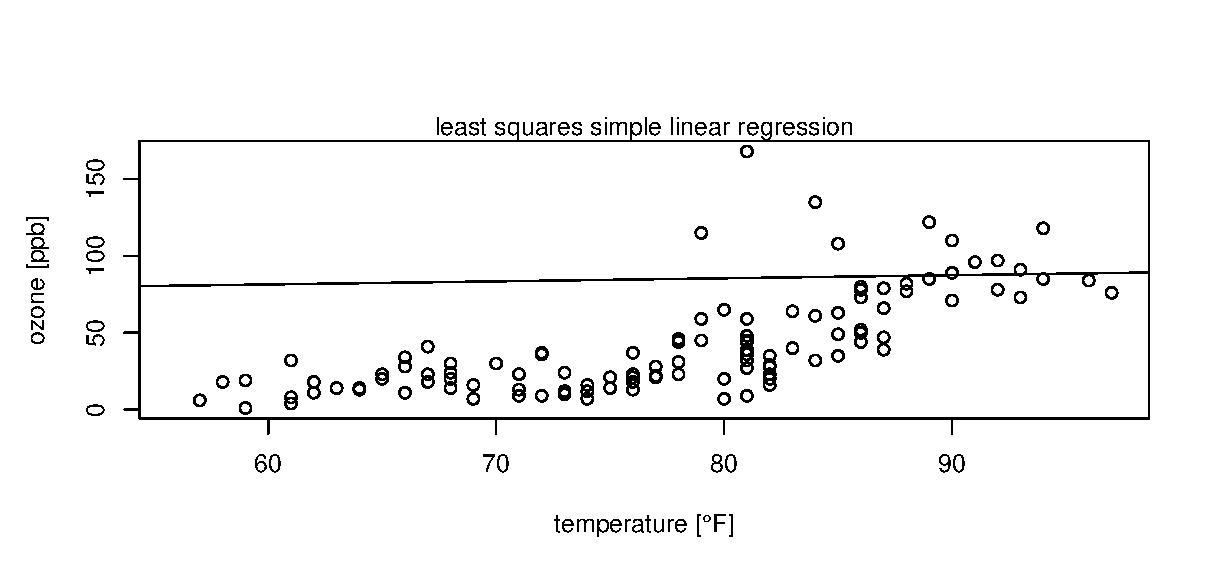
\includegraphics[scale=0.8]{linReg.eps}
\end{center}
\caption{Example of a best-fit linear model obtained by the method
of least squares for the case of the bivariate joint distribution
featured in Fig-~\ref{fig:scatterplot}. The least square estimators
for the $y$-intercept and the slope take values
$a = 69.41~\text{ppb}$ and
$b = 0.20~(\text{ppb}/\text{°F})$, respectively. \newline
\underline{\R:} \newline
\texttt{data("airquality")} \newline
\texttt{?airquality} \newline
\texttt{regMod <- lm( airquality\$Temp~\texttildelow~airquality\$Ozone )} \newline
\texttt{summary(regMod)} \newline
\texttt{plot( airquality\$Temp , airquality\$Ozone )} \newline
\texttt{abline(regMod)}}
\lb{fig:linReg}
\end{figure}
%

\medskip
\noindent
Note that Eq.~(\ref{eq:linregmodel}) may be re-expressed in terms 
of the corresponding $Z$ scores of $X$ and $\hat{Y}$, according to
Eq.~(\ref{eq:standardisationdiscriptive}), to yield
%
\be
\left(\frac{\hat{y}-\bar{y}}{s_{Y}}\right)
= r\left(\frac{x-\bar{x}}{s_{X}}\right)
\qquad\Leftrightarrow\qquad
\hat{z}_{Y} = rz_{X} \ .
\ee
%

%%%%%%%%%%%%%%%%%%%%%%%%%%%%%%%%%%%%%%%%%%%%%%%%%%%%%%%%%%%%%%%%%%%
\section[Coefficient of determination]{Coefficient of
determination}
\lb{sec:bestreg}
%%%%%%%%%%%%%%%%%%%%%%%%%%%%%%%%%%%%%%%%%%%%%%%%%%%%%%%%%%%%%%%%%%%
The quality of any particular simple linear regression model, 
i.e., its \textbf{goodness-of-the-fit}, is assessed by means of the 
\textbf{coefficient of determination} $B$ (metr). This measure is 
derived by starting from the algebraic identity
%
\be
\sum_{i=1}^{n}(y_{i}-\bar{y})^{2}
=\sum_{i=1}^{n}(\hat{y}_{i}-\bar{y})^{2}
+\sum_{i=1}^{n}(y_{i}-\hat{y}_{i})^{2} \ ,
\ee
%
which, upon conveniently re-arranging, leads to defining a quantity
%
\be
\lb{eq:linregcoeffdetdescr}
\fbox{$\displaystyle
B:=\frac{{\displaystyle\sum_{i=1}^{n}(y_{i}-\bar{y})^{2}
-\sum_{i=1}^{n}(y_{i}-\hat{y}_{i})^{2}}}{{\displaystyle
\sum_{i=1}^{n}(y_{i}-\bar{y})^{2}}}
= \frac{{\displaystyle\sum_{i=1}^{n}(\hat{y}_{i}-\bar{y})^{2}}}{
{\displaystyle\sum_{i=1}^{n}(y_{i}-\bar{y})^{2}}} \ ,
$}
\ee
%
with range $0 \leq B \leq 1$. A perfect fit is signified by $B=1$, 
while no fit amounts to $B=0$. The coefficient of determination 
provides a descriptive measure for the proportion of variability 
of $Y$ in a bivariate data set $\{(x_{i},y_{i})\}_{i=1,\ldots,n}$ 
that can be accounted for as due to the association with $X$ via 
the simple linear regression model. Note that in simple linear 
regression it holds that
%
\be
\lb{eq:linregrsq}
B=r^{2} \ ;
\ee
%
see, e.g., Toutenburg (2004) \ct[p~150f]{tou2004}).

\medskip
\noindent
\underline{\R:}
\texttt{summary( lm(\textit{variable:y}~\texttildelow~\textit{variable:x}) )} \\
\underline{EXCEL, OpenOffice:} \texttt{RSQ} (dt.:
\texttt{BESTIMMTHEITSMASS}) \\
\underline{SPSS:} Analyze $\rightarrow$ Regression
$\rightarrow$ Linear \ldots $\rightarrow$ Statistics \ldots: Model 
fit

\vspace{5mm}
\noindent
This concludes Part I of these lecture notes, the introductory 
discussion on uni- and bivariate
\href{https://www.youtube.com/watch?time_continue=2&v=pTtYMdqZ1M4}{\textbf{descriptive statistical methods of data analysis}}. We wish to
encourage the interested reader to adhere to accepted scientific
standards when actively getting involved with data analysis
her/him-self. This entails, amongst other aspects, foremost the
truthful documentation of all data taken into account in a specific
analysis conducted. Features facilitating understanding such as
visualisations of empirical distributions by means of, where
appropriate, histograms, bar charts, box plots or scatter plots, or
providing the values of five number summaries, sample means, sample
standard deviations, standardised skewness and excess kurtosis
measures, or sample correlation coefficients should be commonplace
in any kind of research report. It must be a prime objective of the
researcher to empower potential readers to retrace the inferences
made by her/him.

\medskip
\noindent
To set the stage for the application of inferential statistical
methods in Part III, we now turn to review the elementary concepts
underlying \textbf{Probability Theory}, predominantly as
interpreted in the \textbf{frequentist approach} to this topic.

%%%%%%%%%%%%%%%%%%%%%%%%%%%%%%%%%%%%%%%%%%%%%%%%%%%%%%%%%%%%%%%%%%%
%%%%%%%%%%%%%%%%%%%%%%%%%%%%%%%%%%%%%%%%%%%%%%%%%%%%%%%%%%%%%%%%%%%
